\documentclass[a4paper,12pt]{article}

\usepackage{graphicx}
\usepackage{caption}
\usepackage{subcaption}
\usepackage[utf8]{inputenc}
\usepackage[english,greek]{babel}
\usepackage{hyperref}
\usepackage{amsmath}

\title{Τεχνικές Βελτιστοποίησης - Εργασία 3}
\author{Ρουσομάνης Γεώργιος (ΑΕΜ: 10703)}
\date{Δεκέμβριος 2024}

\begin{document}

\maketitle

\section*{Εισαγωγή}

Στόχος της συγκεκριμένης εργασίας είναι η ελαχιστοποίηση μίας μη γραμμικής συνάρτησης $f(x)$, η οποία υπόκειται σε
περιορισμούς της μορφής $\alpha_i \leq x_i \leq \beta_i$, με τη χρήση της μεθόδου μέγιστης καθόδου με προβολή. 
Η αντικειμενική συνάρτηση που θα μελετηθεί είναι η:
\[
f(x) = \frac{1}{3} x_1^2 + 3 x_2^2, \quad x = \begin{bmatrix} x_1 \\ x_2 \end{bmatrix}.
\]
Η γραφική παράσταση της συνάρτησης παρουσιάζεται στο Σχ.~\ref{fig:objective_function}. 

Τα αποτελέσματα της μεθόδου μέγιστης καθόδου με προβολή θα συγκριθούν με εκείνα της κλασικής μεθόδου μέγιστης καθόδου
χωρίς περιορισμούς. Η ανάλυση θα περιλαμβάνει την επίδραση του βήματος $\gamma_k$ στη σύγκλιση της κλασικής μεθόδου, 
ενώ τα αποτελέσματα της προσομοίωσης στον υπολογιστή θα επαληθευτούν με μαθηματική ανάλυση.

Για τη μέθοδο μέγιστης καθόδου με προβολή, θα εξεταστεί η επίδραση του βήματος $\gamma_k$, της παραμέτρου $s_k$, 
καθώς και του σημείου εκκίνησης στη σύγκλιση της μεθόδου. 

\begin{figure}
    \centering
    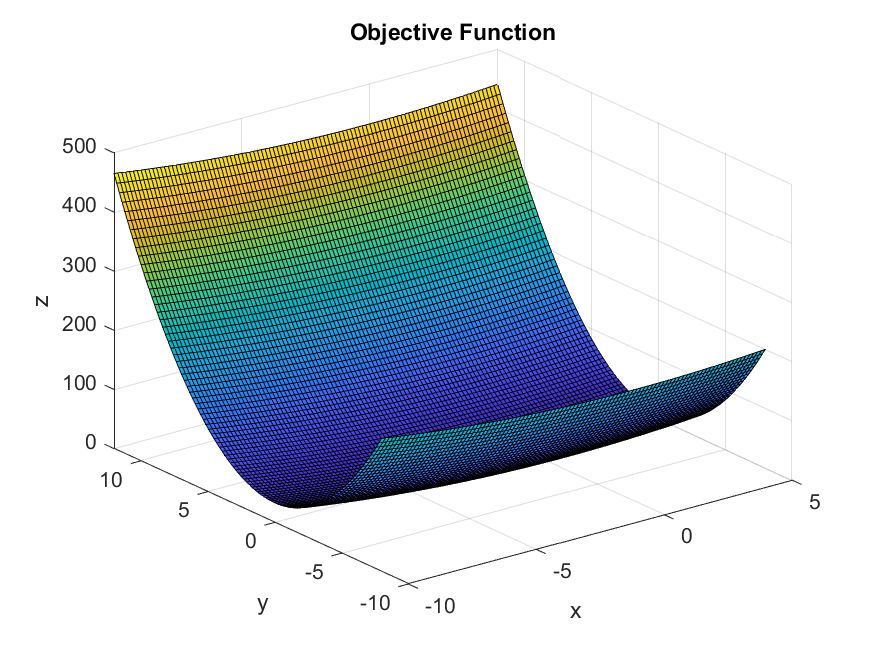
\includegraphics[width=1\linewidth]{plot/objective_function.pdf}
    \caption{Αντικειμενική Συνάρτηση}
    \label{fig:objective_function}
\end{figure}

\section*{Θέμα 1}
Όπως είναι ήδη γνωστό, η μέθοδος μέγιστης καθόδου αποτελεί μια τεχνική βελτιστοποίησης για προβλήματα απουσία 
περιορισμών. Ο αλγόριθμος υπολογίζει διαδοχικά σημεία μέσω της αναδρομικής σχέσης: 
\[
x_{k+1} = x_k - \gamma_k \nabla f(x_k) \implies 
\begin{bmatrix} x_{1(k+1)} \\ x_{2(k+2)} \end{bmatrix} = 
\begin{bmatrix} x_{1k} \\ x_{2k} \end{bmatrix}
 - \gamma_k \begin{bmatrix} \frac{2}{3} x_{1k} \\ 6 x_{2k} \end{bmatrix}
\]

Προφανώς, η $f$ παρουσιάζει ολικό ελάχιστο στο $x^* = (0,0)$. Για να συγκλίνει η μέθοδος για οποιοδήποτε αρχικό
σημείο $x_0 \neq x^*$ θα πρέπει να ισχύει:
\[
\left|\frac{x_{1(k+1)}}{x_{1k}}\right| < 1 \implies \left|1 - \frac{2}{3} \gamma_k \right| < 1 
\implies 0 < \gamma_k < 3
\]
και
\[
\left|\frac{x_{2(k+1)}}{x_{2k}}\right| < 1 \implies \left|1 - 6 \gamma_k \right| < 1 
\implies 0 < \gamma_k < \frac{1}{3}
\]
Από τα παραπάνω προκύπτει ότι για να έχουμε σύγκλιση στο $x^* = (0,0)$ θα πρέπει να ισχύει $0 < \gamma_k < \frac{1}{3}$.

Στο Σχ.~\ref{fig:task1_convergence} παρουσιάζεται το γράφημα σύγκλισης της αντικειμενικής συνάρτησης ως προς τον αριθμό 
των επαναλήψεων με αρχικό σημείο $x_0 = (5, -5)$, για διάφορες τιμές του $\gamma_k$. Παρατηρούμε ότι για $\gamma_k = 0.1$ 
και $\gamma_k = 0.3$ έχουμε επιτυχή σύγκλιση (δεδομένου ότι $\gamma_k < 1/3$), ενώ για $\gamma_k = 3$ και $\gamma_k = 5$
η μέθοδος αποκλίνει (δεδομένου ότι $\gamma_k > 1/3$). Το αποτέλεσμα αυτό συμφωνεί με τα συμπεράσματα της θεωρητικής 
ανάλυσης. Επίσης για $\gamma_k = 0.3$ έχουμε ταχύτερη σύγκλιση από ότι για $\gamma_k = 0.1$.

\begin{figure}[h]
    \centering
    \begin{minipage}{0.47\textwidth}
        \centering
        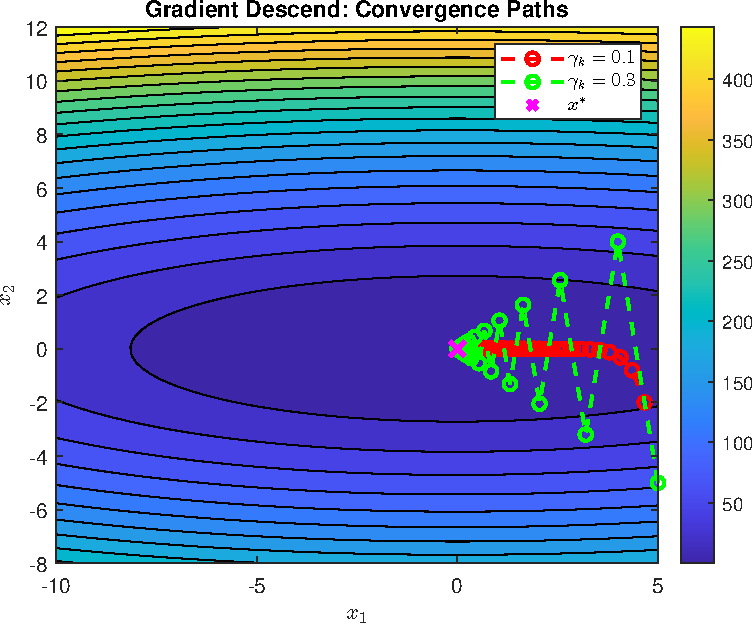
\includegraphics[width=1\linewidth]{plot/task1_contour.pdf}
        \caption{\small Διαδοχικά σημεία υπολογισμού για τις περιπτώσεις σύγκλισης για το Θέμα 1}
        \label{fig:task1_contour}
    \end{minipage} \hfill
    \begin{minipage}{0.47\textwidth}
        \centering
        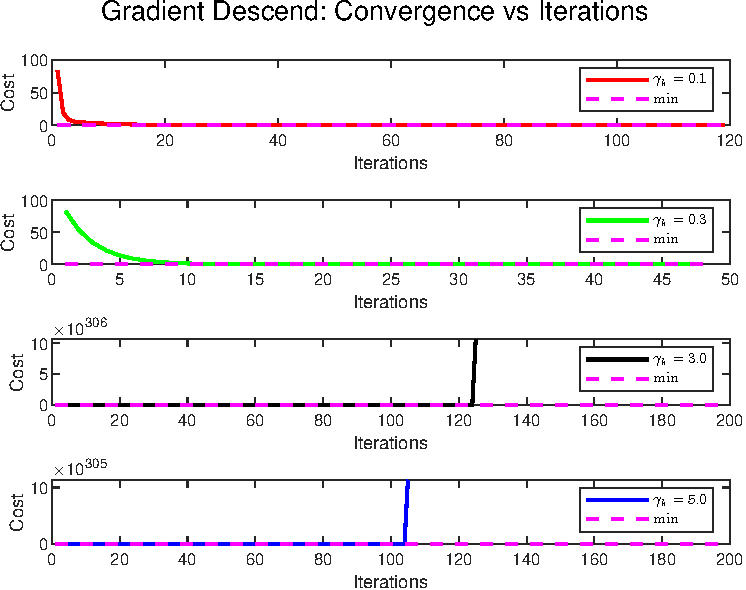
\includegraphics[width=1\linewidth]{plot/task1_convergence.pdf}
        \caption{\small Σύγκλιση της αντικειμενικής συνάρτησης ως προς τον αριθμό των επαναλήψεων για την μέθοδο μέγιστης καθόδου}
        \label{fig:task1_convergence}
    \end{minipage}
\end{figure}


\section*{Θέμα 2}
Η μέθοδος μέγιστης καθόδου με προβολή αποτελλεί μία τεχνική βελτιστοποίησης για προβλήματα με περιορισμούς.
Ο αλγόριθμος υπολογίζει διαδοχικά εφικτά σημεία της μορφής
\[
x_{k+1} = x_k + \gamma_k (\bar{x}_k - x_k), \quad \gamma_k \in (0, 1]
\]
όπου
\[
\bar{x}_k = Pr_X\{x_k - s_k \nabla f(x_k)\}, \quad s_k > 0.
\]
Επομένως, το $\bar{x}_k$ προσδιορίζεται από το $x_k$ αν κινηθούμε στην κατεύθυνση της αρνητικής κλήσης με
βήμα $s_k$ και στην συνέχεια βρούμε την προβολή του $x_k - s_k \nabla f(x_k)$ στο $X$, καταλήγοντας με τον
τρόπο αυτό σε εφικτό σημείο. Έχοντας βρει την εφικτή κατεύθυνση αναζήτησης $\bar{x}_k - x_k$, κινούμαστε με
βήμα $\gamma_k \in (0, 1]$ σ' αυτήν και προσδιορίζουμε το νέο σημείο $x_{k+1}$. Το \(x_{k+1}\) θα είναι 
επίσης εφικτό, καθώς αποτελεί γραμμικό συνδυασμό των $x_k, \bar{x}_k \in X$ με $\gamma_k \in (0, 1]$, 
και $X$ κυρτό σύνολο.
 
Στο Σχ.~\ref{fig:task2_contour} φαίνονται τα διαδοχικά σημεία που υπολογίζει ο αλγόριθμος μέγιστης καθόδου με 
προβολή, με σημείο αφετηρίας $x_0 = (5, -5)$, $s_k = 5$, $\gamma_k = 0.5$ και ακρίβεια $\epsilon = 0.01$. 
Παρατηρούμε ότι εμφανίζεται ταλάντωση γύρω από το $x^*$. Αυτό συμβαίνει διότι $\gamma_k s_k > \frac{1}{3}$. Επίσης,
καθώς ο αλγόριθμος κινείται προς το $x^*$, η κατεύθυνση κίνησης που ορίζεται από το $\bar{x}_k - x_k$ έχει
την τάση να γίνει κάθετη προς την κατεύθυνση που οδηγεί στο ελάχιστο, κάνοντας τον αλγόριθμο ιδιαίτερα 
αναποτελεσματικό.

Στο ίδιο σχήμα βλέπουμε την τροχιά των σημείων που υπολογίζει ο αλγόριθμος για $s_k = 0.6$, $\gamma_k = 0.5$ και
$x_0 = (5, -5)$. Σε αυτήν την περίπτωση έχουμε σύγκλιση της μεθόδου καθώς ισχύει $\gamma_k s_k < \frac{1}{3}$.

Στο Σχ.~\ref{fig:task2_convergence} παρουσιάζεται το γράφημα σύγκλισης της αντικειμενικής συνάρτησης 
συναρτήσει του αριθμού επαναλήψεων. Στην πρώτη περίπτωση (όπου $\gamma_k s_k > \frac{1}{3}$) βλέπουμε ότι η αδυναμία 
σύγκλισης της μεθόδου μέγιστης καθόδου με προβολή οδηγεί σε ταλάντωση της τιμής της αντικειμενικής συνάρτησης καθώς
αυξάνεται το πλήθος των επαναλήψεων. Αυτό είναι αντίθετο με τη συμπεριφορά της κλασικής μεθόδου μέγιστης καθόδου, 
όπου η αδυναμία σύγκλισης οδηγεί σε απειρισμό της αντικειμενικής συνάρτησης. Η παραπάνω διαφορά εξηγείται από το 
γεγονός ότι η μέθοδος μέγιστης καθόδου με προβολή υπολογίζει σημεία μόνο εντός του κυρτού συνόλου $X$, αποτρέποντας 
τον απειρισμό της συνάρτησης.

\begin{figure}[h]
    \centering
    \begin{minipage}{0.47\textwidth}
        \centering
        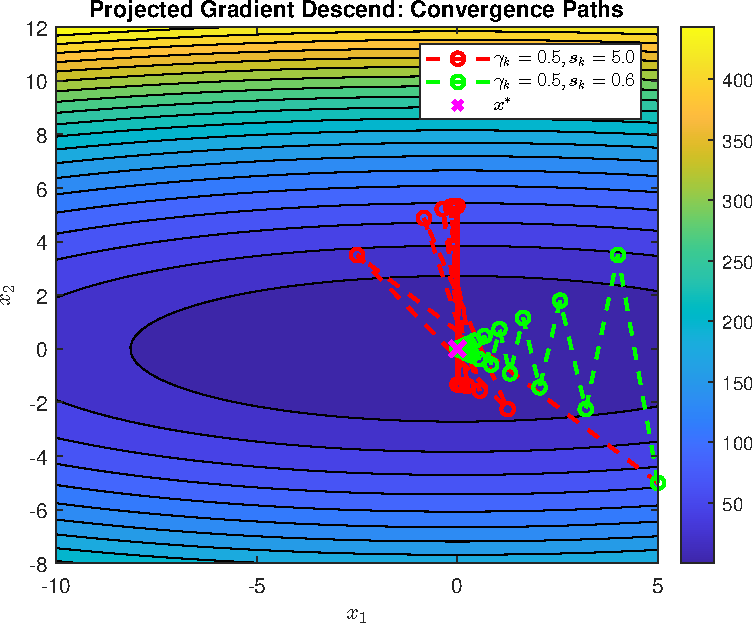
\includegraphics[width=1\linewidth]{plot/task2_contour.pdf}
        \caption{\small Διαδοχικά σημεία υπολογισμού της μεθόδου μέγιστης καθόδου με προβολή για το Θέμα 2}
        \label{fig:task2_contour}
    \end{minipage} \hfill
    \begin{minipage}{0.47\textwidth}
        \centering
        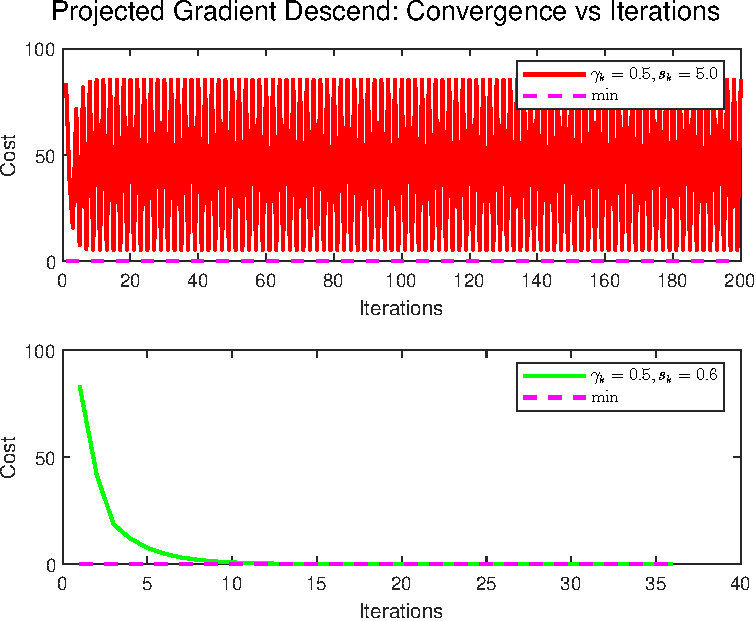
\includegraphics[width=1\linewidth]{plot/task2_convergence.pdf}
        \caption{\small Σύγκλιση της αντικειμενικής συνάρτησης ως προς τον αριθμό των επαναλήψεων για την μέθοδο μέγιστης καθόδου με προβολή για το Θέμα 2}
        \label{fig:task2_convergence}
    \end{minipage}
\end{figure}

\section*{Θέμα 3}
Σε αυτή την περίπτωση θα χρησιμοποιήσουμε την μέθοδο μέγιστης καθόδου με προβολή με $s_k = 15$, $\gamma_k = 0.1$
με σημείο εκκίνησης το $x_0 = (-5, 10)$ και ακρίβεια $\epsilon = 0.01$.

Στο Σχ.~\ref{fig:task3_contour} φαίνεται η τροχία των σημείων που υπολογίζει ο αλγόριθμος. Όπως και στο Θέμα~2, 
παρατηρείται αδυναμία σύγκλισης, καθώς $\gamma_k s_k > \frac{1}{3}$. Ωστόσο, η ταλάντωση που παρουσιάζεται 
έχει πολύ μικρότερο πλάτος, λόγω της μικρότερης τιμής του $\gamma_k$. 

Επιπλέον, από το Σχ.~\ref{fig:task3_convergence} βλέπουμε ότι δεν εμφανίζεται απειρισμός της αντικειμενικής συνάρτησης, 
σε αντίθεση με το Θέμα~1. Όπως έχει ήδη επισημανθεί, αυτό συμβαίνει επειδή ο αλγόριθμος μέγιστης καθόδου με προβολή 
υπολογίζει σημεία εντός του κυρτού συνόλου $X$.

Ένας πρακτικός τρόπος ώστε η μέθοδος να συγκλίνει στο ελάχιστο, είναι η μείωση του $s_k$ ή $\gamma_k$ έτσι ώστε
να ισχύει $\gamma_k s_k < \frac{1}{3}$. Στο Σχ.~\ref{fig:task3_contour} και στο Σχ.~\ref{fig:task3_convergence} 
βλέπουμε την σύγκλιση της μεθόδου για $\gamma_k = 0.1$ και $s_k = 3$.

\begin{figure}[h]
    \centering
    \begin{minipage}{0.47\textwidth}
        \centering
        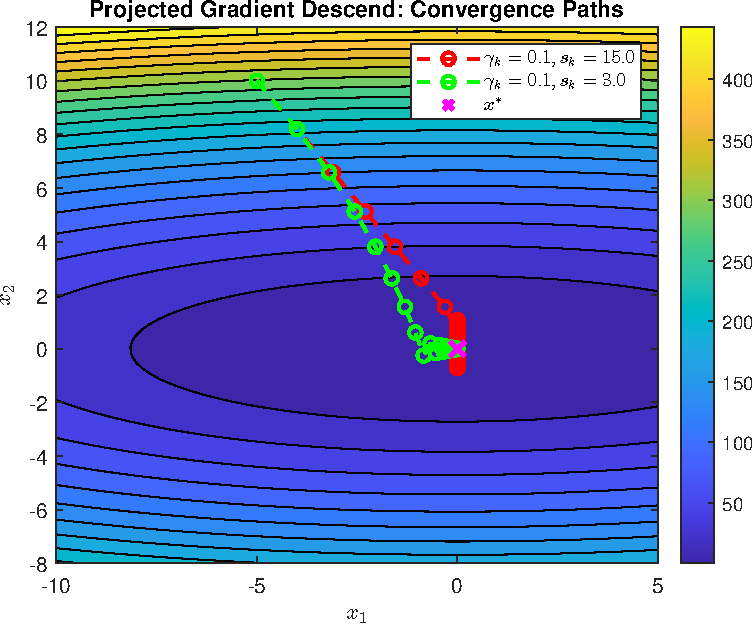
\includegraphics[width=1\linewidth]{plot/task3_contour.pdf}
        \caption{\small Διαδοχικά σημεία υπολογισμού της μεθόδου μέγιστης καθόδου με προβολή για το Θέμα 3}
        \label{fig:task3_contour}
    \end{minipage} \hfill
    \begin{minipage}{0.47\textwidth}
        \centering
        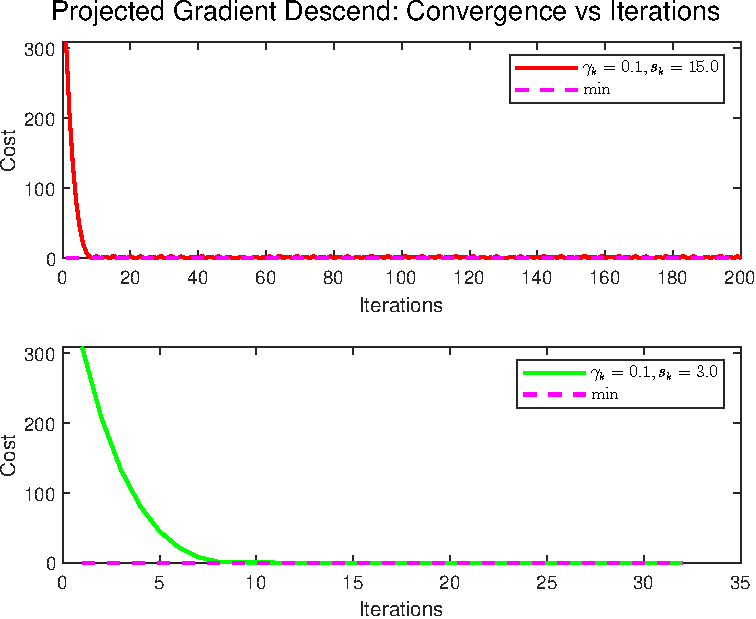
\includegraphics[width=1\linewidth]{plot/task3_convergence.pdf}
        \caption{\small Σύγκλιση της αντικειμενικής συνάρτησης ως προς τον αριθμό των επαναλήψεων για την μέθοδο μέγιστης καθόδου με προβολή για το Θέμα 3}
        \label{fig:task3_convergence}
    \end{minipage}
\end{figure}

\section*{Θέμα 4}
Θα χρησιμοποιήσουμε την μέθοδο μέγιστης καθόδου με προβολή με $s_k = 0.1$, $\gamma_k = 0.2$ με σημείο εκκίνησης το 
$x_0 = (8, -10)$ και ακρίβεια $\epsilon = 0.01$. Σε αυτήν την περίπτωση το σημείο αφετηρίας $x_0$ δεν είναι εφικτό,
οπότε θα αναμέναμε ότι ο αλγόριθμος δεν θα συγκλίνει στο ελάχιστο. Ωστόσο, από το Σχ.~\ref{fig:task4_contour} και το
Σχ.~\ref{fig:task4_convergence} διαπιστώνουμε ότι κάτι τέτοιο δεν ισχύει.

Αυτό μπορεί να εξηγηθεί αν ανατρέξουμε στον τρόπο λειτουργίας της μεθόδου. Σε κάθε επανάληψη, ο αλγόριθμος προβάλλει
το διάνυσμα μέγιστης καθόδου $x_k - s_k \nabla f(x_k)$ στο εφικτό και κυρτό σύνολο $X$. Με αυτόν τον τρόπο διορθώνεται 
η κατεύθυνση κίνησης του σημείου, οδηγώντας το κάθε φορά προς το κοντινότερο σημείο εντός του $X$.

Μόλις το σημείο εισέλθει εντός του $X$, εφόσον ισχύει $\gamma_k s_k < \frac{1}{3}$, ο αλγόριθμος θα συγκλίνει στο 
ελάχιστο. Στα Σχ.~\ref{fig:task4_contour} και Σχ.~\ref{fig:task4_convergence} φαίνεται η αδυναμία σύγκλισης της μεθόδου
όταν θέσουμε $s_k = 2$ έτσι ώστε $\gamma_k s_k > \frac{1}{3}$. Ωστόσο, και σε αυτή την περίπτωση, το σημείο εισέρχεται
εντός του $X$.

Συνεπώς, η χρήση της προβολής επιτρέπει στον αλγόριθμο να ξεπεράσει το αρχικό πρόβλημα του μη εφικτού σημείου εκκίνησης 
και να συγκλίνει κανονικά στο βέλτιστο σημείο εντός των περιορισμών, με την προϋπόθεση ότι $\gamma_k s_k < \frac{1}{3}$.

\begin{figure}[h]
    \centering
    \begin{minipage}{0.47\textwidth}
        \centering
        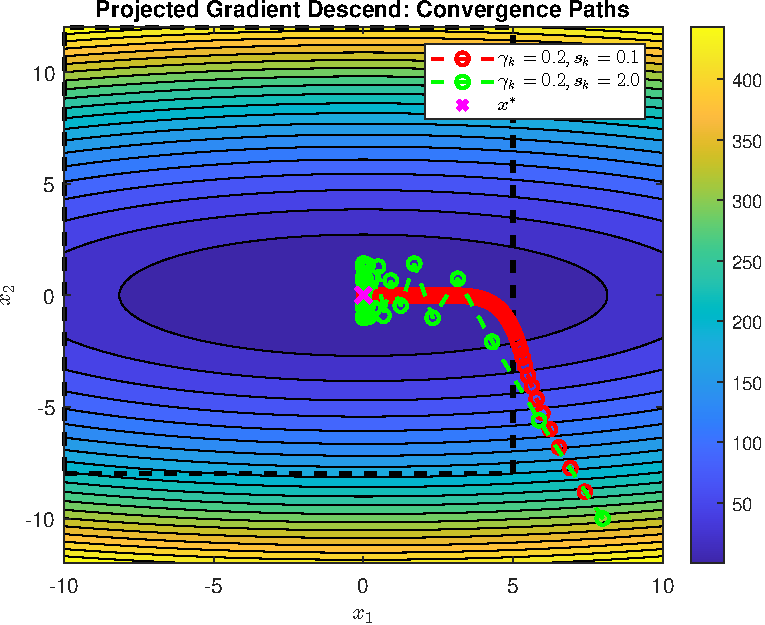
\includegraphics[width=1\linewidth]{plot/task4_contour.pdf}
        \caption{\small Διαδοχικά σημεία υπολογισμού της μεθόδου μέγιστης καθόδου με προβολή για το Θέμα 4}
        \label{fig:task4_contour}
    \end{minipage} \hfill
    \begin{minipage}{0.47\textwidth}
        \centering
        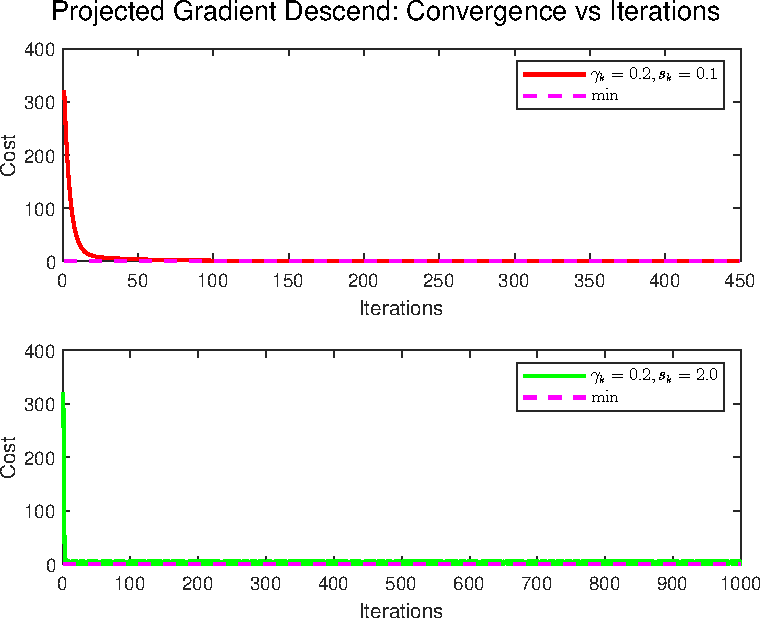
\includegraphics[width=1\linewidth]{plot/task4_convergence.pdf}
        \caption{\small Σύγκλιση της αντικειμενικής συνάρτησης ως προς τον αριθμό των επαναλήψεων για την μέθοδο μέγιστης καθόδου με προβολή για το Θέμα 4}
        \label{fig:task4_convergence}
    \end{minipage}
\end{figure}

\newpage

\section*{Συμπέρασμα}

Από την ανάλυση των αποτελεσμάτων για τη μέθοδο μέγιστης καθόδου και τη μέθοδο μέγιστης καθόδου με προβολή, 
προκύπτουν τα εξής συμπεράσματα:

1. **Μέθοδος Μέγιστης Καθόδου χωρίς Περιορισμούς**:
   - Η σύγκλιση της μεθόδου εξαρτάται από την επιλογή του βήματος $\gamma_k$.
   - Για να εξασφαλιστεί σύγκλιση προς το ελάχιστο της αντικειμενικής συνάρτησης, πρέπει να ισχύει 
     $0 < \gamma_k < \frac{1}{3}$. Εάν $\gamma_k$ είναι μεγαλύτερο, η μέθοδος αποκλίνει.
   - Τα μεγαλύτερα αποδεκτά $\gamma_k$ εντός του παραπάνω διαστήματος ($\gamma_k \approx \frac{1}{3}$) 
     εξασφαλίζουν ταχύτερη σύγκλιση.

2. **Μέθοδος Μέγιστης Καθόδου με Προβολή**:
   - Η μέθοδος είναι κατάλληλη για προβλήματα με περιορισμούς και υπολογίζει διαδοχικά εφικτά σημεία εντός του 
     κυρτού συνόλου $X$.
   - Η σύγκλιση εξαρτάται από τις παραμέτρους $s_k$ και $\gamma_k$, με την προϋπόθεση ότι $\gamma_k s_k < \frac{1}{3}$ 
     για να επιτευχθεί σύγκλιση.
   - Σε περιπτώσεις που η συνθήκη $\gamma_k s_k < \frac{1}{3}$ δεν ισχύει, παρατηρείται ταλάντωση γύρω από το βέλτιστο σημείο, 
     χωρίς όμως να εμφανίζεται απειρισμός της αντικειμενικής συνάρτησης, καθώς τα σημεία παραμένουν εντός του κυρτού συνόλου $X$.

3. **Αντιμετώπιση Μη Εφικτών Σημείων Εκκίνησης**:
   - Η μέθοδος μέγιστης καθόδου με προβολή μπορεί να ξεκινήσει από μη εφικτά σημεία, καθώς η προβολή διασφαλίζει ότι 
     τα επόμενα σημεία υπολογίζονται εντός του κυρτού συνόλου $X$.
   - Αφού το σημείο εκκίνησης εισέλθει στο $X$, η μέθοδος μπορεί να συγκλίνει στο ελάχιστο εφόσον $\gamma_k s_k < \frac{1}{3}$.

4. **Γενικά Συμπεράσματα**:
   - Η μέθοδος μέγιστης καθόδου με προβολή είναι πιο ευέλικτη σε σύγκριση με την κλασική μέθοδο μέγιστης καθόδου, 
     καθώς μπορεί να διαχειριστεί προβλήματα με περιορισμούς και μη εφικτά σημεία εκκίνησης.
   - Ωστόσο, για τη βελτιστοποίηση της απόδοσης, απαιτείται προσεκτική επιλογή των παραμέτρων $s_k$ και $\gamma_k$.
   - Η σωστή προσαρμογή αυτών των παραμέτρων διασφαλίζει γρήγορη και σταθερή σύγκλιση, ενώ αποτρέπει φαινόμενα ταλάντωσης.

Συνολικά, η χρήση των δύο μεθόδων ανάλογα με τη φύση του προβλήματος βελτιστοποίησης προσφέρει σημαντικά εργαλεία 
για την επίλυση τόσο μη περιορισμένων όσο και περιορισμένων προβλημάτων με υψηλή ακρίβεια.


\end{document}
